\chapter{Diagnostics}\label{app:Diagnostics}

The dedicated pedestal experiments, both in I-mode and ELMy H-mode, presented here required an extensive suite of diagnostics to characterize pedestal behavior.  Broadly, these diagnostics may be broken down into three categories:

\begin{description}
 \item[Thomson Scattering] \hfill \\
 Details the edge Thomson scattering diagnostic, from which the high-resolution profile data used for the bulk of this thesis was gathered.
 \item[Fast Diagnostics] \hfill \\
 Details the Electron-Cyclotron Emission (ECE) and $H_\alpha$ line radiation diagnostics used to track sawtooth crashes and ELM events in the plasma edge.
 \item[Fluctuation Diagnostics] \hfill \\
 Details Gas-Puff Imaging (GPI), Reflectometry, and other diagnostics used to characterize the mid-frequency fluctuations found in I-mode pedestals.\nicesectionending
\end{description}

\section{Thomson Scattering}\label{sec:app_ts}

Due to the steep gradients in density, temperature, and pressure found in the pedestal, accurate characterization of plasma profiles in this region requires diagnostics capable of very fine spatial resolution.  Measurements based on the Thomson scattering \cite{Sheffield} of laser light off of electrons in the plasma provides the high-resolution pedestal profiles used in this thesis: Thomson scattering is a near-direct measurement of electron temperature and density, independent of bulk plasma parameters (\ie it is unaffected by the cutoffs or reflections found in other diagnostics, and produces no significant perturbation to the plasma).  Measurement via Thomson scattering produces an effective ``snapshot'' of the plasma parameters at each measurement point, with spatial resolution limited only by collection optics geometry, and time resolution limited by repetition rate on the lasers.  Despite significant technical difficulties -- for example, the high-powered lasers and sensitive collection optics needed 
to capture the weak scattered light and the necessity for careful calibration of density measurements -- Thomson scattering diagnostics remain a versatile and powerful tool for plasma pedestal measurement, and provided the bulk of the profile data used in this thesis.

\subsection{Principles of Thomson Scattering}\label{subsec:app_background}

An intuitive picture of the Thomson scattering phenomenon may be obtained by the consideration of a stationary, free electron with an EM wave impinging on it.  The particle will be accelerated by the wave (approximately sinusoidally for $E$-field-dominated acceleration at nonrelativistic speeds), causing it to radiate.  Any motion of the electron will cause Doppler shifting in the scattered radiation -- motion relative to the incident wave shifts the incident frequency $\omega_i$, at which the particle oscillates, while motion relative to an observer shifts the scattered wave.  This geometry for general positions of the particle and observer is given in \cref{fig:app_ts_geometry}.

\begin{figure}[t]
 \pushtooutside
 \ffigbox[\FBwidth]{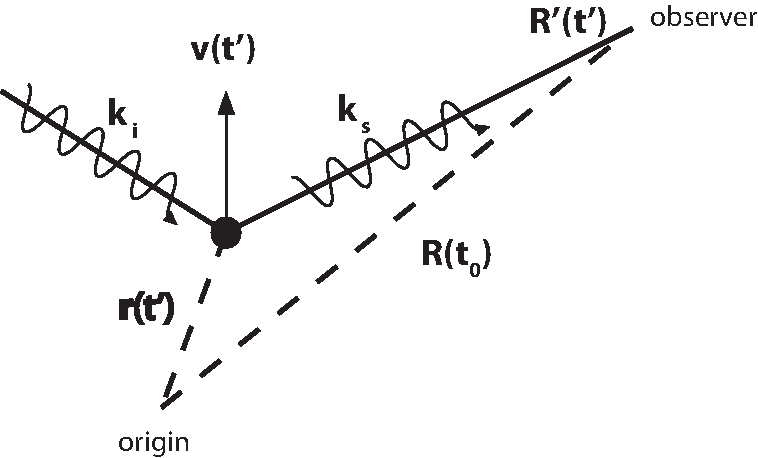
\includegraphics[width=150mm]{graphics/Diagnostics/TS_geometry.pdf}}{\caption{Coordinate system considered for Thomson scattering, with the incident wave of wavenumber $\vec{k}_i$ incident on a particle at $\vec{r}(t')$ for retarded time $t'$.  The scattered wave $\vec{k}_s$ is drawn to an observer at $\vec{R}(t')$.}\label{fig:app_ts_geometry}}
\end{figure}

The scattered electric field from a generally-accelerated electron moving at $\vec{\beta} = \vec{v}/c$ is given from the Lienard-Wiechert potentials \cite[\S 7]{Hutchinson},

\begin{equation}\label{eq:LienardWiechert}
 \begin{gathered}
  \vec{E}_s = \frac{-e}{4\pi\varepsilon_0} \left\llbracket \frac{1}{\kappa^3 Rc} \hat{s} \times \left( \left(\hat{s} \times \vec{\beta}\right) \times \dot{\beta}\right)\right\rrbracket_{t'}\\
  \kappa = 1 = \frac{\vec{R}' \cdot \vec{v}}{R'c} = 1 - \hat{s} \cdot \vec{\beta}, \qquad t' = t - \frac{R'}{c}
  \end{gathered}
\end{equation}

\noindent where $\hat{s}$ indicates the unit vector along the scattering direction, $\vec{R} = R\hat{s}$ is the vector to the observer, $\kappa$ is a relativistic scale factor, and $t'$ is the relativistic retarded time.  The apostrophe indicates a parameter evaluated at the retarded time, \ie $R' = R(t')$; the bracketed term in \cref{eq:LienardWiechert} likewise is evaluated at $t'$.  The scattered power per solid angle is given by

\begin{equation}\label{eq:dPdOmega}
 \begin{aligned}
  \frac{dP_s}{d\Omega} &= R^2 \vec{S}\cdot\hat{s} = R^2 \frac{1}{\mu_0} \left(\vec{E} \times \vec{B}\right)\cdot\hat{s}\\
  &= R^2 \varepsilon_0 c \left(\vec{E}_s \times \left(\hat{s} \times \vec{E}_s\right)\right) \cdot \hat{s} = R^2 c \varepsilon_0 \left|E_s\right|^2
 \end{aligned}
\end{equation}

\noindent Relativistically, the electron motion (which in turn sets the field determined by \cref{eq:LienardWiechert}) is given by

\begin{equation}\label{eq:betadot}
 \dot{\beta} = \frac{d}{dt}\left(\gamma m_e \vec{v}\right) = -e\left(\vec{E}_i + \vec{v} \times \vec{B}_i\right)
\end{equation}

\noindent thus

\begin{equation}\label{eq:betadot2}
 m_e \gamma \dot{\beta} + \gamma^3 m_e \beta \left(\vec{\beta}\cdot\dot{\beta}\right) = -e \left(\frac{\vec{E}_i}{c} + \vec{\beta}\times\vec{B}_i\right)
\end{equation}

\noindent Dotting $\vec{\beta}$ into this and substituting,

\begin{equation}\label{eq:betadot3}
 \dot{\beta} = -\frac{e}{m_e \gamma} \left( \frac{\vec{E}_i}{c} - \frac{\vec{\beta}\cdot\vec{E}_i}{c} \vec{\beta} + \vec{\beta} \times \vec{B}_i \right)
\end{equation}

\noindent The general relativistic solution to \cref{eq:LienardWiechert,eq:dPdOmega} with the above is rather intractible, although full relativistic treatments have been undertaken \cite{Sheffield1972,Matoba1978,Selden1980,Naito1993}.  However, the radiated field may be simplified substantially in the nonrelativistic limit -- in the limit of $\beta \ll 1$, the acceleration is simply

\begin{equation}\label{eq:betadot_nonrel}
 \dot{\beta} = -\frac{e}{m_e c}\vec{E}_i
\end{equation}

\noindent and the scattered field is

\begin{equation}\label{eq:LW_nonrel}
 \vec{E}_s = \frac{e^2}{4\pi\varepsilon_0 m_e c^2} \left\llbracket \frac{1}{R} \hat{s} \times \left(\hat{s}\times\vec{E}_i\right)\right\rrbracket_{t'}
\end{equation}

\noindent Recalling the classical electron radius,

\begin{equation}\label{eq:re}
 r_e = \frac{e^2}{4\pi \varepsilon_0 m_e c^2}
\end{equation}

\noindent the radiated power is given by

\begin{equation}\label{dPdOmega2}
 \frac{dP_s}{d\Omega} = r_e^2 c \varepsilon_0 E_{i0}^2 \left\llbracket \hat{s} \times \left( \hat{s} \times \hat{E}_i \right) \right\rrbracket^2 \cos^2 \left( \vec{k}_i \cdot \vec{r}' - \omega_i t' \right)
\end{equation}

\noindent separating the magnitude, direction, and phase (evaluated at $t'$) of the incident field.

\begin{figure}[t]
 \pushtooutside
 \ffigbox[\FBwidth]{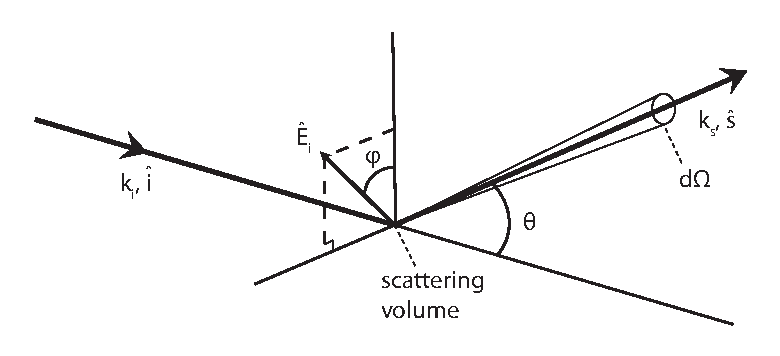
\includegraphics[width=150mm]{graphics/Diagnostics/ts_geometry2.pdf}}{\caption{Definitions of the angular dependences in the Thomson scattering geometry: namely, the angle $\theta$ between the incident wave direction $\hat{i}$ and scattering direction $\hat{s}$, and the polarization angle $\phi$ of the incident electric field $\hat{E}_i$ with respect to the projection of $\hat{s}$ into the polarization plane.}\label{fig:app_ts_geometry2}}
\end{figure}

We may first consider the scattering direction dependence,

\begin{equation}
 \left\llbracket \hat{s} \times \left( \hat{s} \times \hat{E}_i \right) \right\rrbracket^2_{t'}
\end{equation}

\noindent Defining the angular geometry as in \cref{fig:app_ts_geometry2} for the scattering angle $\theta$ between the incident wave direction $\hat{i}$ and scattering direction $\hat{s}$, and the polarization angle $\phi$ (defined between $\hat{E}_i$ and the projection of $\hat{s}$ into the polarization plane), this reduces to (cf. \cite[\S 1.7]{Sheffield})

\begin{equation}
 \left\llbracket \hat{s} \times \left( \hat{s} \times \hat{E}_i \right) \right\rrbracket^2 = 1 - \sin^2 \theta \cos^2 \phi
\end{equation}

\noindent Since the incident power flux is given by

\begin{equation}
 S_i = c \varepsilon_0 E_{i0}^2 \cos^2 \left( \vec{k}_i \cdot \vec{r}' - \omega_i t' \right)
\end{equation}

\noindent We may separate the incident flux and scattering by

\begin{equation}\label{eq:ts_crosssection}
 \frac{dP}{d\Omega} = S_i \frac{d\sigma_t}{d\Omega} \Rightarrow \frac{d\sigma_t}{d\Omega} = r_e^2 [1 - \sin^2 \theta \cos^2 \phi]
\end{equation}

\noindent defining a scattering cross-section $\sigma_t$.  Integrating over $d\Omega$,

\begin{equation}\label{eq:sigmat}
 \sigma_t = \frac{8\pi}{3} r_e^2 = \SI{6.65e-29}{\square\meter}
\end{equation}

\noindent The extremely small cross-section for Thomson scattering necessitates high-powered lasers and sensitive collection optics -- for example, the fraction of photons scattered from a segment along the laser beam path of length $L$ with electron density $n_e$ is given simply by $Ln_e \sigma_t$.  For $L = \SI{1}{\milli\meter}$ and $n_e = \SI{1e20}{\per\cubic\meter}$, Thomson scattering faces an attenuation factor on the order of $\sim 10^{-11}$ to the incident photon count from the laser.

The phase of the scattered wave is determined by a retarded-time evaluation of the incident phase, $\vec{k}_i \cdot \vec{r}(t') - \omega_i t'$.  Substituting $\vec{r}(t') = \vec{r}_0 + \vec{v}t'$, and assuming $R(t') \approx R(t_0)$ (which holds for observers far from the scattering volume, $R \gg r$) we may rewrite the retarded time as

\begin{equation}
 t' = \frac{1}{1 - \hat{s} \cdot \vec{\beta}} \left( 1 - \frac{R}{c} + \frac{\hat{s} \cdot \vec{r}_0}{c} \right)
\end{equation}

\noindent Substituting, the phase argument becomes

\begin{equation}\label{eq:ts_phase}
 k_i \frac{1 - \hat{i} \cdot \vec{\beta}}{1 - \hat{s} \cdot \vec{\beta}} R - \omega_i \frac{1 - \hat{i} \cdot \vec{\beta}}{1 - \hat{s} \cdot \vec{\beta}} t - k_i \frac{1 - \hat{i} \cdot \vec{\beta}}{1 - \hat{s} \cdot \vec{\beta}} \hat{s} \cdot \vec{r}_0 + \vec{k}_i \cdot \vec{r}_0
\end{equation}

\noindent where $\hat{i}$ is the incident wave propagation direction.  We have naturally arrived at the Doppler-shifted frequency, 

\begin{equation}\label{eq:doppler}
 \begin{aligned}
  \omega_s &= \frac{1 - \hat{i} \cdot \vec{\beta}}{1 - \hat{s} \cdot \vec{\beta}} \omega_i\\
  \vec{k}_s &= k_i \frac{1 - \hat{i} \cdot \vec{\beta}}{1 - \hat{s} \cdot \vec{\beta}} \hat{s} = \frac{\omega_s}{c} \hat{s}
 \end{aligned}
\end{equation}

\noindent so the phase is

\begin{equation}
 \vec{k}_i \cdot \vec{r}' - \omega_i t' = k_s R - \omega_s t + \left( \vec{k}_s - \vec{k}_i \right) \cdot \vec{r}_0
\end{equation}

\noindent Alternately, we may define

\begin{equation}\label{eq:ts_komega}
 \begin{aligned}
  \vec{k} &= \vec{k}_s - \vec{k}_i\\
  \omega &= \omega_s - \omega_i = \vec{k} \cdot \vec{v}
 \end{aligned}
\end{equation}

We may establish the frequency spectrum of the scattered radiation by taking the Fourier transform of the scattered field,

\begin{equation}
 \vec{E}_s(\omega_s) = \int \vec{E}_s(t) e^{i\omega_s t} \;dt
\end{equation}

\noindent At retarded time, $dt = \kappa' dt'$, and

\begin{equation}\label{eq:Fourier}
 \vec{E}_s(\omega_s) = \frac{r_e}{R'} \int \kappa' \Pi \cdot \vec{E}_i(\vec{r}',t') e^{- \omega_s \left( t' + \frac{R'}{c} - \frac{\hat{s}\cdot\vec{r}'}{c}\right)} \;dt'
\end{equation}

\noindent Here, for generality we use the polarization tensor $\Pi$, which includes relativistic effects -- in the nonrelativistic limit $\Pi = \hat{s}\hat{s} - \textbf{I}$ such that $\Pi \cdot \vec{E}_i = \hat{s} \times \left( \hat{s} \times \vec{E}_i \right)$.  Using $\vec{E}_i(\vec{r},t) = \vec{E}_{i0} \;\mbox{exp}(i(\vec{k}_i \cdot \vec{r} - \omega_i t))$ and \cref{eq:ts_komega},

\begin{equation}
 \vec{E}_s(\omega_s) = \frac{r_e}{R'} e^{ik_s R'} \int \kappa' \left( \Pi \cdot \hat{E}_i \right) E_{i0} e^{i(\omega t' - \vec{k} \cdot \vec{r}')} \;dt'
\end{equation}

\noindent Integrating and substituting $\omega_s = 2\pi \nu_s$,

\begin{equation}
 \vec{E}_s (\nu_s) = \frac{r_e}{R} e^{ik_s R} 2\pi \kappa \left(\Pi \cdot \vec{E}_{i0}\right) \delta(\vec{k}\cdot\vec{v} - \omega)
\end{equation}

\noindent We may thus construct the scattered power per solid angle per unit frequency

\begin{equation}\label{eq:ts_powerspectrumsingle}
 \frac{d^2 P}{d\Omega d\nu_s} = r_e^2 \left| \Pi \cdot \hat{E}_i \right|^2 \left( c \varepsilon_0 E_{i0}^2 \right) \delta \left( \nu_s - \frac{1 - \hat{i} \cdot \vec{\beta}}{1 - \hat{s} \cdot \vec{\beta}} \nu_i \right)
\end{equation}

\noindent So we have established the scattered power spectrum in solid angle and frequency of a single electron as a function of scattering direction (encoded in $\Pi \cdot \hat{E}_i$) and incident laser energy( in the incident Poynting flux $\langle S_i \rangle = c \varepsilon_0 E_{i0}^2$).  The scattered spectrum locked to a single frequency by the Dirac delta function, forcing the scattered spectrum to radiate strictly at the Doppler-shifted frequency set by the electron motion.

To consider the spectrum from a population of electrons, we must consider the interactions between nearby electrons.  On length scales comparable to the electron Debye length $\lambda_{De}$ (\cref{eq:debye}), electrons in the plasma screen out incident electric fields -- this organized motion leads to interference in the scattered radiation, referred to as \emph{collective} or \emph{coherent scattering}.  The full solution for the scattered spectrum (see \cite[\S 3]{Sheffield}) may be expanded in a series in the factor

\begin{equation}\label{eq:ts_alpha}
 \alpha = \frac{1}{k\lambda_{De}}
\end{equation}

\noindent Coherent effects are negligible in the limit of $\alpha \ll 1$, at which the scattering is said to be \emph{incoherent} or \emph{noncollective} -- the radiation from a population of electrons is simply the sum of each individual contribution.  For the effective scattering wavevector, $\vec{k} = \vec{k}_s - \vec{k}_i$ (\cref{eq:ts_komega}),

\begin{equation}
 \begin{aligned}
 \left| \vec{k} \right| &= \sqrt{k_s^2 + k_i^2 - 2k_s k_i \cos \theta}\\ &\approx \sqrt{2} k_i \sqrt{1 - \cos \theta} = \sqrt{2} k_i \sqrt{2 \sin^2 \left(\frac{\theta}{2}\right)}
 \end{aligned}
\end{equation}

\noindent assuming $k_s \approx k_i$.  Thus the noncollective requirement reduces to

\begin{equation}\label{eq:ts_incoherent}
 \frac{1}{2k_i \sin(\theta/2) \lambda_{De}} \ll 1 \Rightarrow \frac{\lambda_i}{\lambda_{De}} \ll 4\pi \sin \left(\frac{\theta}{2}\right)
\end{equation}

\noindent This condition is readily satisfied at near-perpendicular scattering ($\theta \approx \SI{90}{\degree}$, where the scattering amplitude is maximized) and with laser wavelengths much smaller than the Debye length ($\lambda_{De} \sim 10-100 \;\si{\micro\meter}$ at tokamak conditions, compared to the $\lambda_i \sim \SI{1}{\micro\meter}$ IR lasers commonly used for Thomson scattering photon sources).

Thus, the incoherent scattered spectrum is simply the sum of contributions from each electron in the scattering volume -- the spectrum from a population described by the distribution function $f_e(\vec{r},\vec{v})$ is

\begin{equation}\label{eq:ts_powerspectrumint}
 \frac{d^2 P}{d\Omega d\nu_s} = 2\pi r_e^2 \int_{V} \langle S_i \rangle \int \left| \Pi \cdot \hat{E}_i \right|^2 f_e(\vec{r},\vec{v}) \kappa^2 \delta(\vec{k} \cdot \vec{v} - \omega) \;d^3 \vec{v} d^3 \vec{r}
\end{equation}

\noindent For small scattering volumes, the electron distribution function is approximately uniform in space.  In the nonrelativistic limit, $\Pi \cdot \hat{E}_i$ is independent of velocity, thus the spatial contribution may be separated out:

\begin{equation}
 \int_V \langle S_i \rangle \left| \Pi \cdot \hat{E}_i \right|^2 \;d^3 \vec{r}
\end{equation}

\noindent encoding the incident photon flux (from the Poynting vector of the laser) and the scattering direction dependence.  The velocity integral (noting $\kappa \approx 1$ in the nonrelativistic case) is

\begin{equation}
 \int f(\vec{v}) \, \delta(\vec{k} \cdot \vec{v} - \omega) \;d^3 \vec{v}
\end{equation}

\noindent Splitting the velocity into components parallel and perpendicular to $\vec{k}$, $\vec{v}_\perp$, $\vec{v}_k$, this is

\begin{equation}
 \int f(\vec{v}_\perp,\vec{v}_k) \, \delta(kv_k - \omega) \;d^2 \vec{v}_\perp dv_k = \int f_k(v_k) \,\delta(kv_k - \omega) d\vec{v}_k
\end{equation}

\noindent utilizing the normalization required for $f(\vec{v})$ to solve the integrals over $\vec{v}_\perp$.  For a Maxwellian (\cref{eq:maxwell}) the distribution along the effective wavevector $\vec{k}$ is

\begin{equation}\label{eq:ts_fk}
 f_k(v_k) = n_e \frac{1}{v_t \sqrt{\pi}} e^{-v_k^2/v_t^2}
\end{equation}

\noindent thus the above is solvable,

\begin{equation}
 \int f_k(v_k) \,\delta(kv_k - \omega) \;dv_k = \frac{1}{k} f_k\left(\frac{\omega}{k}\right)
\end{equation}

\noindent Substituting into \cref{eq:ts_powerspectrumint},

\begin{equation}\label{eq:ts_powerspectrimint2}
 \begin{aligned}
 \frac{d^2 P}{d\Omega d\nu_s} = &2\pi r_e^2 \left[ \int_V \langle S_i \rangle \left| \hat{s} \times \left( \hat{s} \times \hat{E}_i \right) \right|^2 \;d^3 \vec{r} \right] \times\\ &\frac{1}{\sqrt{\pi}k} \frac{n_e}{v_t} \;\mbox{exp}\left(-\frac{\omega^2}{k^2 v_t^2} \right)
 \end{aligned}
\end{equation}

\noindent Substituting $k \approx 2k_i \sin(\theta/2) = \left(4\pi/\lambda_i\right) \sin(\theta/2)$, the exponent is

\begin{equation}\label{eq:ts_exp}
 -\frac{(\omega_s - \omega_i)^2}{4\dfrac{4\pi^2}{\lambda_i^2} \sin^2 \left(\theta/2\right) v_t^2} \approx -\frac{c^2 (\lambda_s - \lambda_i)^2}{4\lambda_i^2 v_t^2 \sin^2(\theta/2)}
\end{equation}

\noindent Converting from a frequency to a wavelength spectrum, and assuming the scattering volume to be sufficiently small that the scattering angle and incident Poynting flux are uniform (thus $\int \langle S_i \rangle \;d^3\vec{r} = \langle S_i \rangle AL = P_i L$ for laser cross-section $A$, scattering volume $L$, and laser power $P_i$) the nonrelativistic scattering spectrum is

% \begin{equation}\label{eq:ts_spectrum_nonrel}
%  \begin{aligned}
%  \frac{d^2 P}{d\Omega d\lambda_S} = &P_i r_e^2 n_e L \left| \hat{s} \times \left( \hat{s} \times \hat{E}_i \right) \right|^2 \frac{1}{2\sqrt{\pi} \sin(\theta/2)} \times\\ &\frac{c}{\lambda_i v_t} \;\mbox{exp}\left(-\frac{c^2 (\lambda_s - \lambda_i)^2}{4v_t^2 \lambda_i^2 \sin^2 (\theta/2)}\right)
%  \end{aligned}
% \end{equation}

\begin{equation}\label{eq:ts_spectrum_nonrel}
 \begin{aligned}
  \frac{d^2 P}{d\Omega d\lambda_s} &= P_i r_e^2 n_e L \left| \hat{s} \times \left( \hat{s} \times \hat{E}_i \right) \right|^2 S(T_e, \theta, \lambda_s)\\
  S(T_e,\theta,\lambda_s) &= \frac{1}{2\sqrt{\pi} \sin(\theta/2)} \frac{c}{\lambda_i v_t} \;\mbox{exp}\left(-\frac{c^2 (\lambda_s - \lambda_i)^2}{4v_t^2 \lambda_i^2 \sin^2 (\theta/2)}\right)
 \end{aligned}
\end{equation}

\noindent This expression is a Maxwellian centered at $\lambda = \lambda_i$ with a spread determined by the electron temperature $T_e$ (manifesting in the thermal velocity $v_t$) and the scattering angle $\theta$.  Recalling the angle $\phi$ defined between the incident polarization $\hat{E}_i$ and the scattering direction $\hat{s}$\gnote{ref to figure}, $\left|\hat{s} \times \left( \hat{s} \times \hat{E}_i \right) \right|^2 = \sin^2 \phi$ is maximized for scattering perpendicular to the incident laser polarization.

This analysis breaks down for relativistic electron populations.  However, relativistic effects (see \cite[\S 9]{Sheffield}) may be expressed as a polynomial correction to \cref{eq:ts_spectrum_nonrel},

% \begin{equation}\label{eq:ts_spectrum_rel}
%  \left. \frac{d^2 P}{d\Omega d\lambda_s} \right|_{rel} = \frac{d^2 P}{d\Omega d\lambda_s} \left[ 1 - \frac{3.5(\lambda_s - \lambda_i)}{\lambda_i} + \frac{c^2 (\lambda_s - \lambda_i)^3}{4v_t^2 \lambda_i^2 \sin^2 (\theta/2)}\right]
% \end{equation}

\begin{equation}\label{eq:ts_spectrum_rel}
 S_{rel}(T_e,\theta,\lambda_s) = S(T_e,\theta,\lambda_s) \left[ 1 - \frac{3.5(\lambda_s - \lambda_i)}{\lambda_i} + \frac{c^2 (\lambda_s - \lambda_i)^3}{4v_t^2 \lambda_i^2 \sin^2 (\theta/2)}\right]
\end{equation}

\begin{figure}[t]
 \pushtooutside
 \fcapside[70mm]{\caption{Spectral functions normalized to density and laser power, evaluated at $\theta = \phi = \pi/2$.  The spectrum spreads farther from the laser line at higher temperature, as well as blue-shifting due to relativistic effects.}\label{fig:app_ts_spectrum}}{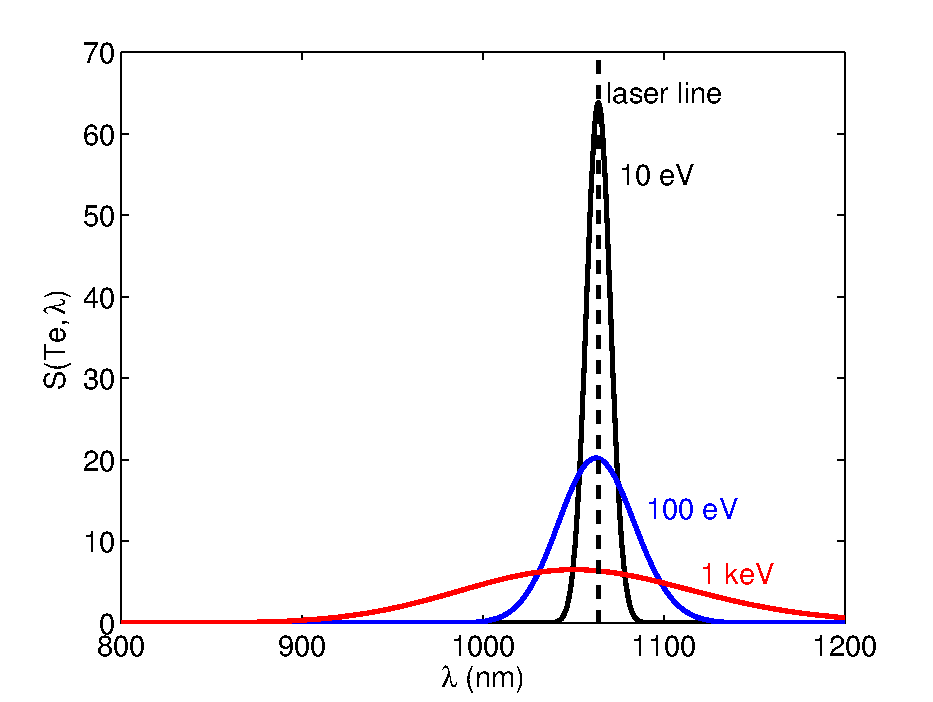
\includegraphics[width=110mm]{graphics/Diagnostics/ts_spectrum.pdf}}
\end{figure}

\noindent The relativistic correction breaks the symmetry of the Maxwellian spectrum, introducing a net blue shift to the spectrum.  Physically, this is due to ``relativistic headlighting,'' in which the radiation from an accelerating relativistic particle is biased forward of its motion -- The radiated power is stronger from particles moving toward the observer (thus with a blue Doppler shift to their emissions).  The spectral form factor $S(T_e,\theta,\lambda_s)$ is shown in figure \cref{fig:app_ts_spectrum}, illustrating the width dependence of the spectrum on the electron temperature and the blue shifting evident in the spectrum even at relatively low plasma temperatures.

Examination of \cref{eq:ts_spectrum_nonrel,eq:ts_spectrum_rel} readily illustrates the method for extracting $n_e$ and $T_e$ measurements from the Thomson scattering spectrum -- the spread of the spectrum of scattered radiation is directly tied to the electron temperature, while the integrated amplitude gives electron density (as the total scattered power is linearly proportional to $n_e$).  Assumptions regarding the Maxwellian distribution of the electrons allows accurate measurement of the electron profile with relatively simple hardware, detailed in the next section.

\subsection{Edge Thomson Scattering on C-Mod}\label{subsec:app_ts_cmod}

In addition to the core Thomson scattering diagnostic \cite{Watterson1990,Mossessian1999}

\begin{figure}[p]
 \pushtooutside
 \ffigbox[\FBwidth]{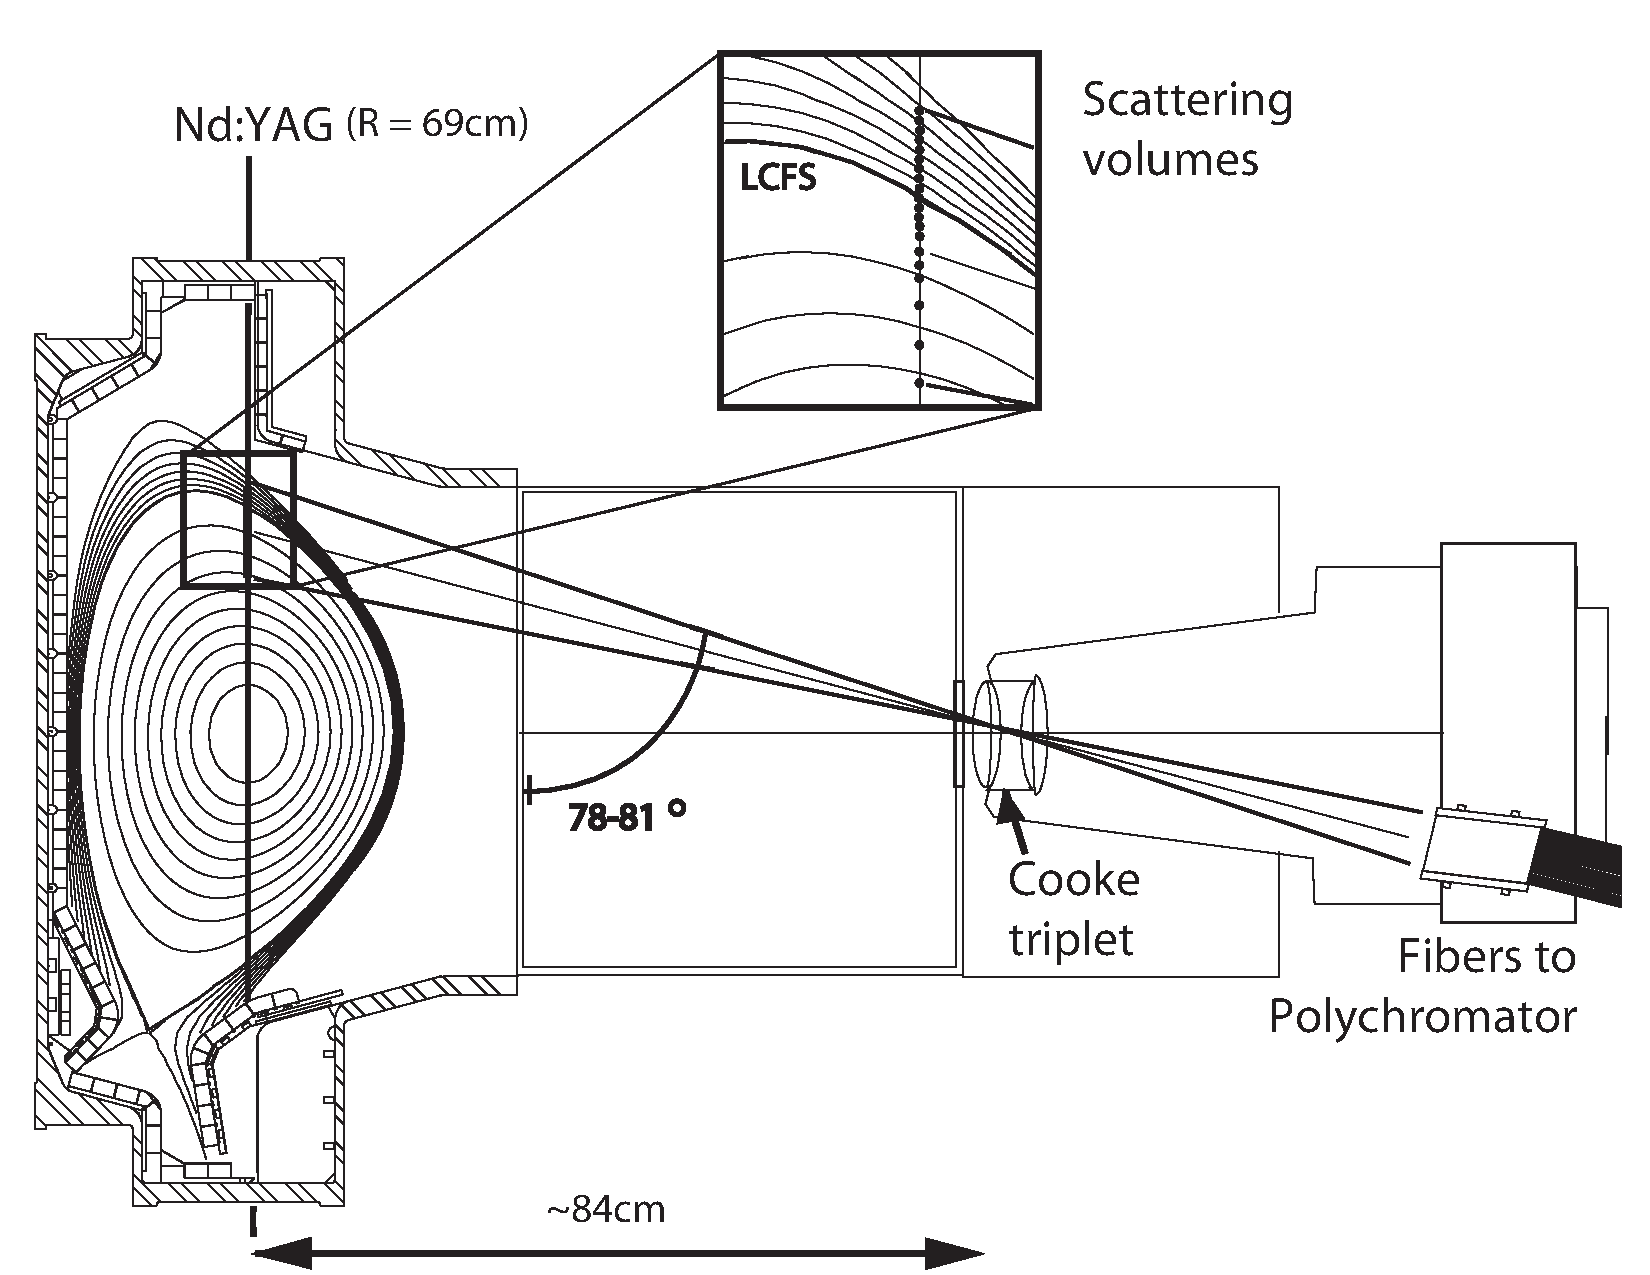
\includegraphics[height=150mm,angle=-90]{graphics/Diagnostics/ts_optics.pdf}}{\caption{Layout of collection optics for the core and edge Thomson scattering diagnostics on Alcator C-Mod.  Two Nd:YAG lasers are fired vertically through the plasma near the magnetic axis, with the scattered light focused through a Cooke triplet at the outboard midplane onto an array of fiber optics.    The positions of the high-resolution edge scattering volumes are highlighted in the inset.}\label{fig:app_ts_optics}}
\end{figure}


\nicesectionending

\section{Fast Diagnostics}\label{sec:app_fast}

\nicesectionending

\section{Fluctuation Diagnostics}\label{sec:app_fluct}

\nicechapterending

\bibliographystyle{../plainurl}
\bibliography{../references}